\chapter{Desenvolvimento}
Etapas do trabalho:
\begin{itemize}
    \item Desenvolvimento e testes do Oscilador em Anel para o Cyclone IV: 2 semanas
    \item Desenvolvimento e testes do Oscilador em Anel para o Kintex-7: 2 semanas
    \item Validação dos circuitos desenvolvidos: 1 semana
    \item Medidas antes do envelhecimento: 2 semanas
    \item Ensaios de envelhecimento acelerado: A etapa mais demorada e variável do trabalho, pois é a que apresenta mais incógnitas no desenvolvimento: 10 semanas
    \item Medidas depois do envelhecimento e análise de dados: 2 semanas
    \item Escrita da monografia: 8 semanas
\end{itemize}

Cronograma:
\begin{figure}[H]
    \centering
    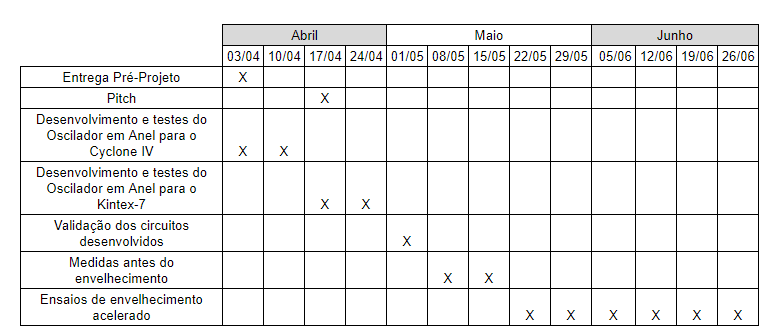
\includegraphics[width=\linewidth]{figures/Cornograma 1.png}
    \label{fig:Cornograma1}
\end{figure}

\begin{figure}[H]
    \centering
    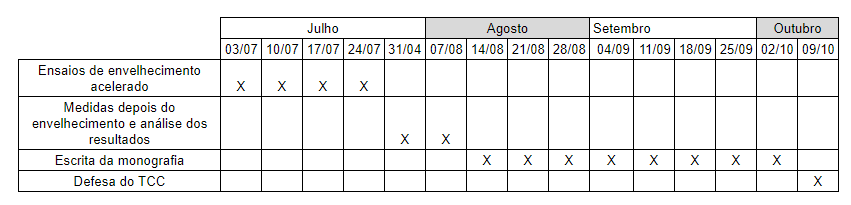
\includegraphics[width=\linewidth]{figures/Cornograma 2.png}
    \label{fig:Cornograma2}
\end{figure}
